% !TeX root = ./l4proj.tex
% REMEMBER: You must not plagiarise anything in your report. Be extremely careful.

\documentclass{l4proj}

    
%
% put any additional packages here
%
\usepackage{graphicx}
\usepackage{subcaption}


\begin{document}

%==============================================================================
%% METADATA
\title{Why is This Sensitive? Visualising Important Sensitivity Classification Features}
\author{Guillaume de Susanne d'Epinay}
\date{\today}

\maketitle

%==============================================================================
%% ABSTRACT
\begin{abstract}
    Every abstract follows a similar pattern. Motivate; set aims; describe work; explain results.
    \vskip 0.5em
    ``XYZ is bad. This project investigated ABC to determine if it was better. 
    ABC used XXX and YYY to implement ZZZ. This is particularly interesting as XXX and YYY have
    never been used together. It was found that  
    ABC was 20\% better than XYZ, though it caused rabies in half of subjects.''
\end{abstract}

%==============================================================================

% EDUCATION REUSE CONSENT FORM
% If you consent to your project being shown to future students for educational purposes
% then insert your name and the date below to  sign the education use form that appears in the front of the document. 
% You must explicitly give consent if you wish to do so.
% If you sign, your project may be included in the Hall of Fame if it scores particularly highly.
%
% Please note that you are under no obligation to sign 
% this declaration, but doing so would help future students.
%
%\def\consentname {My Name} % your full name
%\def\consentdate {20 March 2018} % the date you agree
%

\def\consentname{Guillaume de Susanne d'Epinay}
\def\consentdate{\today}

\educationalconsent


%==============================================================================
\tableofcontents

%==============================================================================
%% Notes on formatting
%==============================================================================
% The first page, abstract and table of contents are numbered using Roman numerals and are not
% included in the page count. 
%
% From now on pages are numbered
% using Arabic numerals. Therefore, immediately after the first call to \chapter we need the call
% \pagenumbering{arabic} and this should be called once only in the document. 
%
% Do not alter the bibliography style.
%
% The first Chapter should then be on page 1. You are allowed 40 pages for a 40 credit project and 30 pages for a 
% 20 credit report. This includes everything numbered in Arabic numerals (excluding front matter) up
% to but excluding the appendices and bibliography.
%
% You must not alter text size (it is currently 10pt) or alter margins or spacing.
%
%
%==================================================================================================================================
%
% IMPORTANT
% The chapter headings here are **suggestions**. You don't have to follow this model if
% it doesn't fit your project. Every project should have an introduction and conclusion,
% however. 
%
%==================================================================================================================================
\chapter{Introduction}

% reset page numbering. Don't remove this!
\pagenumbering{arabic}

\section{The need for Technology Assisted Sensitivity Review}



Motivations
why senstivity review
why technological problem



\section{Objectives}



\section{overview}

bulle tpoi t of chapter ocntent


%==================================================================================================================================
\chapter{Background}

Macdonald et al papers


need for explanations in ML

related products

Document visualization techniques and elaborate on why didnt choose them
"people have done this"

%==================================================================================================================================
\chapter{Requirements}

\section{Scope}

\section{(non)Functional definition}

user study


%==================================================================================================================================
\chapter{Design}

link back to requirements

choice of technologies

\section{Application Structure and Technology stack}

\section{Machine Learning Model}

\section{API}

\section{Frontend}

%==================================================================================================================================
\chapter{Implementation}

show coponennt code and how it gets data from backend

show lime explanations generation

key "features" code overview


\begin{itemize}
    \item Hands on SkLearn framework, experimented with different text pre-processing techniques and classifiers to build a Pipeline to classify textual documents into either sensitive or not sensitive categories
    \item overview of Machine Learning model explanation techniques, successfully implemented the Lime explainer, tried to use the SHAP explainer, but was unsuccessful
    \item Explore text document storage, looked at Terrier, ElasticSearch to finally settle on MongoDB
    \item Packaged SkLearn classifier into Python Flask API with OpenAPI specification
    \item created Javascript API Client from code generated from OpenAPI specification
    \item hands on ReactJS Javascript frontend framework, implemented a document browsing, viewing and upload frontend
    \item added text redaction feature to mark sections as sensitive with a label explaining why it is deemed sensitive
    \item implemented Lime Model explanations in Python backend, exposed them to the Flask API and created a frontend "in text" visualization of these sensitivities
    \item Research Document visualization techniques (literature review)
    \item created a populator script to load and classify all documents
    \item graph visualization of feature contribution to the classification and other UI tweaks
\end{itemize}

%==================================================================================================================================
\chapter{Evaluation}

A user evaluation was conducted to evaluate the effectiveness of the application for reviewing sensitive documents. 

An important consideration in the decisions that follow is that we did not have access to professional document reviewers, as such the evaluation was conducted with students in the role of reviewers. 
% TODO can you really say ground truth for sensitivity?
Our document collection's ground truth for sensitivity was established with respect to sections 40 (International Relations) and 27 (Personal Information) of the Freedom of Information Act (FOIA).
Out test reviewers were asked to identify sensitivities according to section 27 of the FOIA since our reviewers are not experts, finding Personal Information in a document is easier than identifying sensitivites harming International Relations (Section 40).

Due to time constraints we only selected short documents to show our reviewers, that is, documents under 2000 characters. 
We selected both sensitive and non-sensitive documents in order to represent every category of the confusion matrix for the classifier with the following counts:
% TODO update with actual document selection
\begin{table}[h]
    \begin{tabular}{l ll}
                                & Actually non-sensitive & Actually Sensitive \\ 
        Predicted non-sensitive & 3                      & 1                  \\
        Predicted Sensitive     & 1                      & 1                 
    \end{tabular}
    \caption{Document selection in the classifier's confusion matrix}
    \label{tab:confusion-matrix-selection}
\end{table}


\section{Preparations and Experimental Setup}

Multiple interfaces were required to evaluate the effectiveness o


\begin{figure}[h]
    \centering
    \begin{subfigure}[b]{0.7\textwidth}
        \centering
        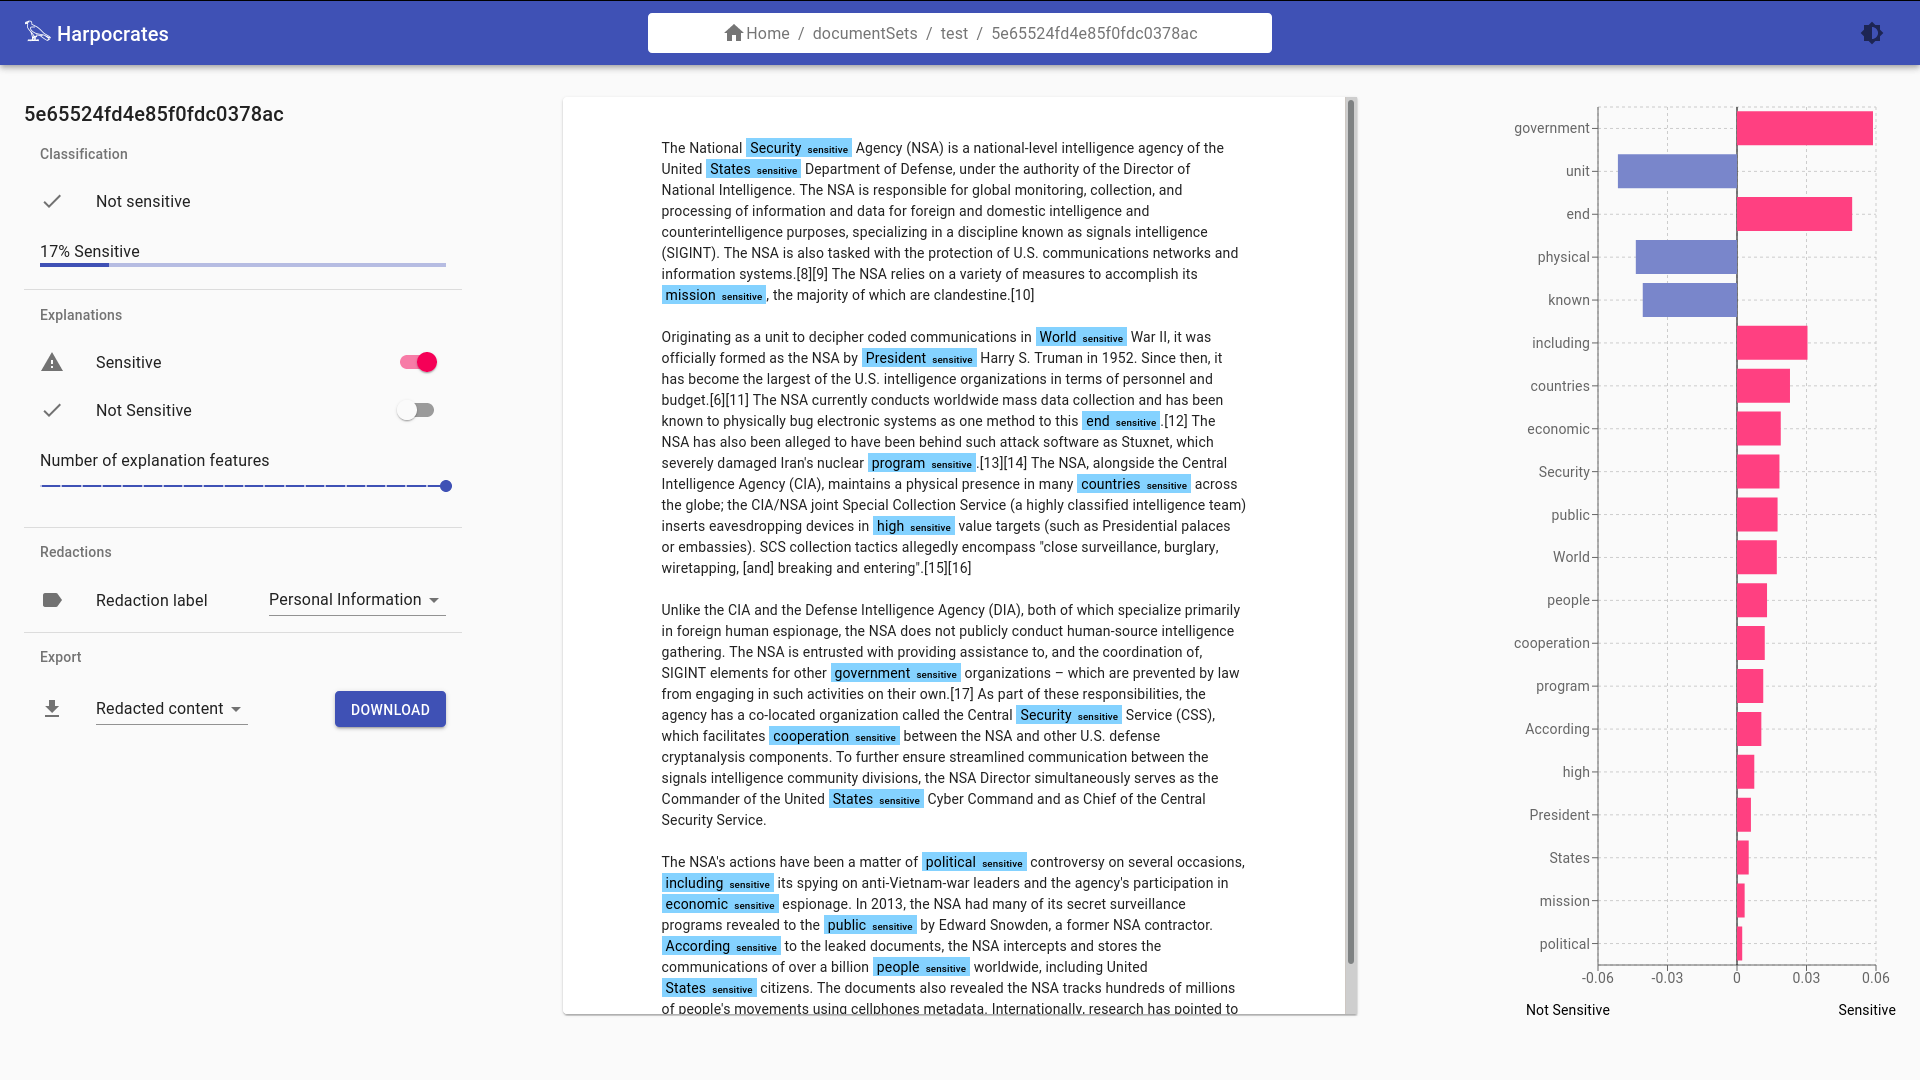
\includegraphics[width=\linewidth]{images/ui_test_mode_1.png}
        \caption{Test mode 1}
        \label{fig:test_mode_1}
    \end{subfigure}
    
    
    \begin{subfigure}[b]{0.7\textwidth}
        \centering
        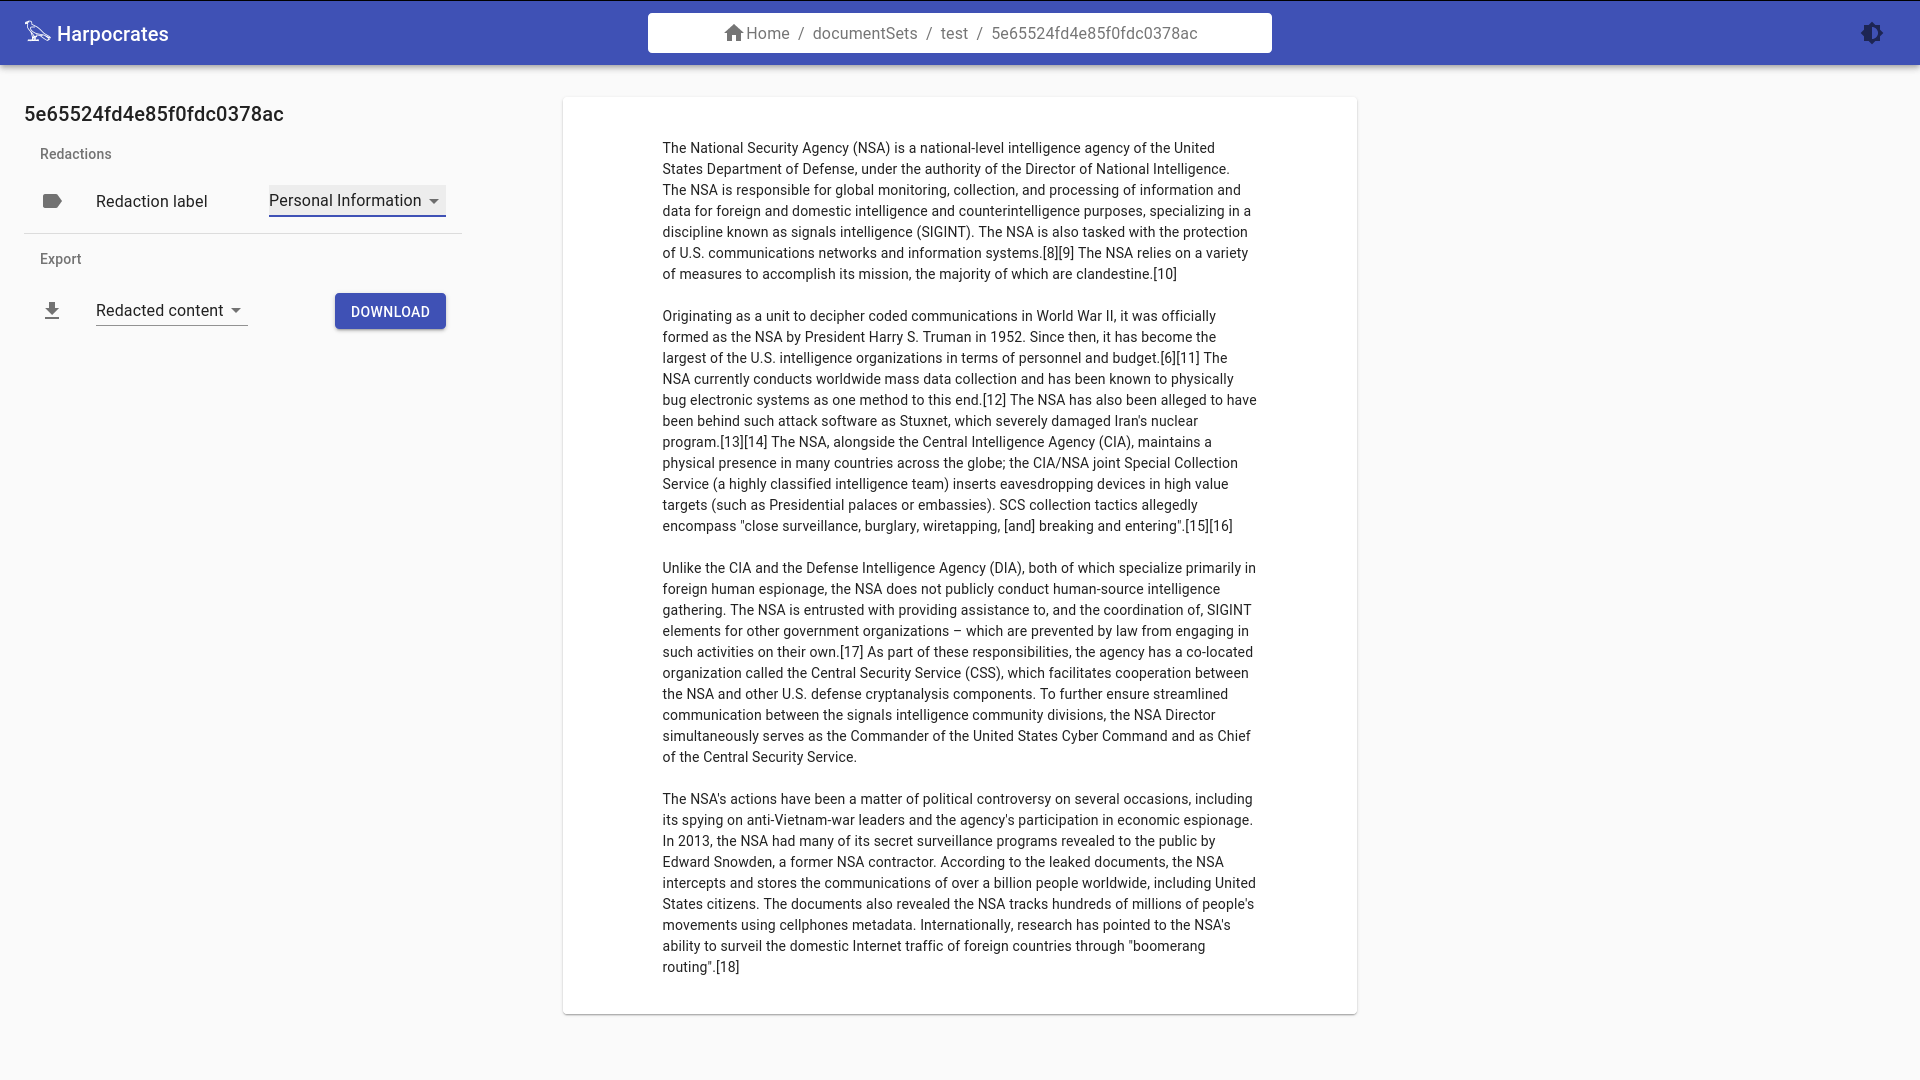
\includegraphics[width=\linewidth]{images/ui_test_mode_2.png}
        \caption{Test mode 2}
        \label{fig:test_mode_2}
    \end{subfigure}
    \caption{The two test modes used for evaluation}
    \label{fig:test_modes}
\end{figure}



\section{Guidance}

Research questions
dependent/indepdent variables
UI variations
experimental setup
document, subject seleciton


results


link back to requirements 
how have they been met
unit testing




%==================================================================================================================================
\chapter{Conclusion}


requirements I've met


reflections 

future work

%==================================================================================================================================
%
% 
%==================================================================================================================================
%  APPENDICES  

\begin{appendices}

    \chapter{Appendices}
    
    Typical inclusions in the appendices are:
    
    \begin{itemize}
        \item
              Copies of ethics approvals (required if obtained)
        \item
              Copies of questionnaires etc. used to gather data from subjects.
        \item
              Extensive tables or figures that are too bulky to fit in the main body of
              the report, particularly ones that are repetitive and summarised in the body.
              
        \item Outline of the source code (e.g. directory structure), or other architecture documentation like class diagrams.
              
        \item User manuals, and any guides to starting/running the software.
              
    \end{itemize}
    
    \textbf{Don't include your source code in the appendices}. It will be
    submitted separately.
    
\end{appendices}

%==================================================================================================================================
%   BIBLIOGRAPHY   

% The bibliography style is abbrvnat
% The bibliography always appears last, after the appendices.

\bibliographystyle{abbrvnat}

\bibliography{l4proj}

\end{document}
